\documentclass{article}

\PassOptionsToPackage{numbers,compress}{natbib}
\usepackage[dblblindworkshop]{neurips_2026}
\workshoptitle{On-Device Intelligence: Foundation Models under Real-World Constraints}

\usepackage[utf8]{inputenc}
\usepackage[T1]{fontenc}
\usepackage{hyperref}
\usepackage{url}
\usepackage{booktabs}
\usepackage{amsfonts}
\usepackage{amsmath}
\usepackage{nicefrac}
\usepackage{microtype}
\usepackage{xcolor}
\usepackage{graphicx}
\usepackage{multirow}
\usepackage{xspace}

\graphicspath{{figures/}}
\newcommand{\system}{\textsc{PhaseGate}\xspace}
\newcommand{\fixed}[1]{\textsc{Fixed}-#1}
\newcommand{\gate}[2]{\textsc{PhaseGate} $#1{\rightarrow}#2$}
\newcommand{\tpot}{\textsc{TPOT}\xspace}
\newcommand{\ttft}{\textsc{TTFT}\xspace}
\newcommand{\qps}{\textsc{QPS}\xspace}

\title{PhaseGate: Phase-Aware CPU Retrieval Scheduling for On-Device LLMs on Unified Memory}
\author{Anonymous Author(s)}

\begin{document}
\maketitle

\begin{abstract}
On-device assistants increasingly run GPU-based LLM inference alongside CPU tasks such as retrieval, indexing, and tool execution on the same unified-memory system.
Under a saturated local-retrieval workload, four concurrent searches raise 95th-percentile (p95) decode latency by 60--61\% on two M4 systems, whereas prefill latency rises by only 5.7--6.9\%.
A conventional scheduler applies one retrieval-concurrency limit throughout an LLM request; that limit must remain safe during sensitive decode and therefore leaves CPU capacity unused during safer prefill.
On our base-M4 configuration, one concurrent search satisfies the latency limits, but two do not.
\system instead calibrates separate limits for prefill and decode, selecting four and one, respectively, on this configuration.
It achieves $2.0\times$ the latency-constrained retrieval throughput of the best tested feasible fixed policy while meeting both latency limits in every evaluation run.
A phase-blind control uses the same high and low limits for the same fractions of wall-clock time but switches independently of the actual LLM phase; it achieves similar raw retrieval throughput yet violates the output-token limit in every run.
M2 and M2 Pro Mac minis reproduce the policy ordering, while output-length sweeps show that the advantage narrows as decode occupies more of each request.
\end{abstract}

\section{Introduction}

Compact models now power Apple Intelligence and Gemini Nano on mobile devices~\cite{gunter2024apple,geminiteam2023gemini}.
Yet an assistant also performs retrieval, contextual-memory lookup, indexing, parsing, and tool execution on the CPU.
Representative agentic applications spend substantial time in CPU-side tools~\cite{raj2025cpu}, and on-device vector-search systems must coordinate interactive queries with background ingestion and index maintenance~\cite{zhao2026muse}.

Retrieval-augmented generation and agent memory embed documents or memories, find vectors similar to a query, and add the matches to the LLM prompt~\cite{apple2025rag}.
We use Hierarchical Navigable Small World (HNSW), a common approximate nearest-neighbor graph implemented in FAISS~\cite{malkov2020hnsw,johnson2021faiss}.
This representative search kernel, not a complete agent workflow, performs irregular pointer chasing instead of a dense scan.

Server accelerators stream model state from GPU-local high-bandwidth memory (HBM), separate from host DRAM used by CPU tools~\cite{nvidia2022h100,zhong2024distserve}.
Apple Silicon instead exposes CPU and GPU to unified memory~\cite{apple2020m1}, making CPU pointer chasing and GPU weight streaming compete for memory service.
Prior integrated-SoC work throttles CPU traffic~\cite{ali2018bwlock}, but does not ask \emph{when} overlap is safer.

LLM phase supplies that signal: prefill processes prompt tokens in parallel and reuses weight loads, whereas decode emits one token at a time and repeatedly streams model state.
On a fanless M4 MacBook Air, four HNSW searches increase p95 time-to-first-token (TTFT), our prefill-sensitive metric, by 5.7\%, but time-per-output-token (TPOT), our decode metric, by 61\%; a fan-cooled base-M4 Mini preserves the direction.
Section~\ref{sec:observation} defines this saturated workload and shows why CPU byte rate alone misses the risk.

A conventional retrieval pool uses one maximum concurrency throughout an LLM request; our Fixed policies model this phase-oblivious baseline.
On the primary M4, Fixed-1 meets both latency limits, while the faster Fixed-2 violates output-token latency.
\system instead calibrates separate prefill and decode limits (Figure~\ref{fig:overview}) and selects 4$\rightarrow$1: four searches during prefill, but one during decode.
This pair is deployment-specific, and we compare it with a phase-blind timer that alternates the same limits without observing LLM phase.

\begin{figure}[t]
  \centering
  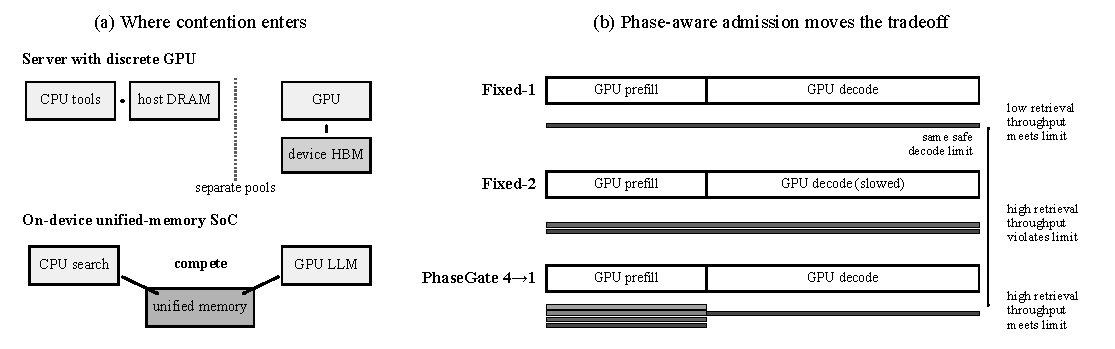
\includegraphics[width=\linewidth]{phasegate_overview.pdf}
  \caption{(a) Server GPU HBM is distinct from CPU host DRAM; an on-device CPU and GPU share one pool.
(b) On the measured base-M4 configuration, Fixed-1 meets both latency limits but restricts retrieval; Fixed-2 retrieves more but violates the output-token limit.
Calibrated \system 4$\rightarrow$1 keeps the safe decode limit while using four-way prefill concurrency.
Schematic.}
  \label{fig:overview}
\end{figure}

\paragraph{Contributions.} (1) We establish prefill--decode asymmetry using HNSW on two M4 systems and four access patterns on M4/M1 Airs.
(2) We design \system to preserve a safe decode limit while using higher prefill concurrency; a time-matched phase-blind control isolates phase alignment.
(3) We evaluate the scheduler on M4, M2, and M2 Pro Minis and vary output length.

\section{Observation: Phase-Asymmetric Interference}
\label{sec:observation}

\paragraph{Experimental Setup.}
We co-run Qwen2.5-1.5B at 4-bit in MLX-LM~\cite{qwen2025} with a read-only FAISS HNSW index (100,000 384-dimensional vectors; graph connectivity $M=32$); LLM requests use 2,048 input and 128 output tokens.
Each worker handles one single-threaded query, so limit four permits at most four independent searches.
We keep the query queue nonempty to measure the maximum sustainable retrieval throughput under an LLM-latency constraint.
This saturated capacity experiment represents waiting batched or cross-session searches, not a typical single-user trace or prerequisite retrieval that finishes before its own request.
Under intermittent arrivals, the queue is often empty and both contention and \system's benefit shrink.

\paragraph{Decode Is Much More Sensitive.}
On the M4 Mini, we first measure LLM latency without retrieval, then allow one, two, or four concurrent HNSW searches.
Each search setting uses 300 LLM requests and three repetitions; the one-, two-, and four-search settings run in randomized order.
TTFT captures the prompt-processing delay, while TPOT captures the pace of output-token generation.
With two concurrent searches on the M4 Mini, p95 TTFT increases by only 1.3\%, whereas p95 TPOT increases by 31\%.
With four, Figure~\ref{fig:mechanism}a shows 5.7\% versus 61\% on the Air and 6.9\% versus 60\% on the Mini; the Mini shows greater decode sensitivity in every repetition.
This pattern is consistent with prefill amortizing weight reads while decode has little reuse.

\paragraph{Access Pattern Matters Too.}
We compare HNSW pointer chasing with bulk STREAM/\allowbreak memcpy, a contiguous sequential scan, and an address-jumping random gather.
Across the three controls, p95 decode slowdown is 27--43\% on M4 and 21--43\% on M1, versus only 4.0--6.0\% and 0.90--3.5\% for prefill.
On M4, a 2.4~GB/s random gather slows decode by 29\%, more than a 51~GB/s scan; M1 preserves the ordering (26\% versus 21\%).
Thus access pattern and LLM phase are distinct axes: byte rate alone is a poor proxy, and pattern-aware admission could further distinguish scan-like from pointer-chasing work such as HNSW~\cite{malkov2020hnsw}.

\begin{figure}[t]
  \centering
  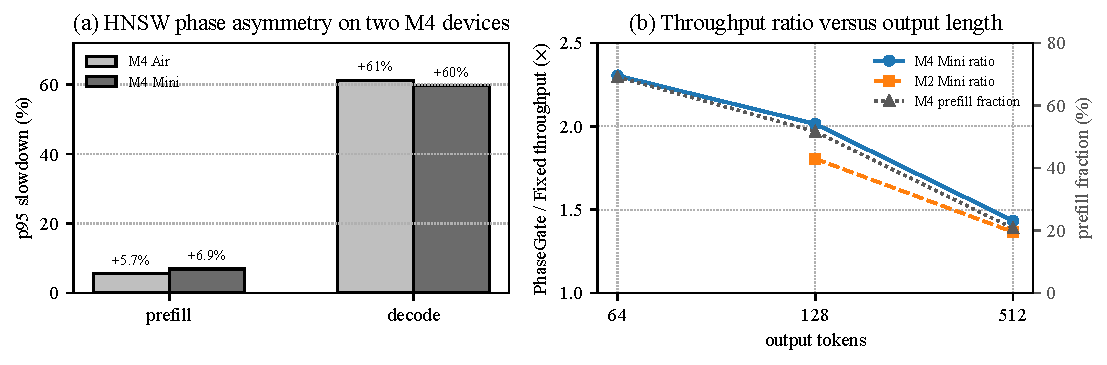
\includegraphics[width=\linewidth]{mechanism_and_sensitivity.pdf}
  \caption{(a) Four concurrent HNSW searches show the same p95 asymmetry on a fanless M4 Air and fan-cooled base-M4 Mini; each Mini bar is the median of three runs with 300 LLM requests per run.
(b) PhaseGate/Fixed throughput falls with output length on base-M4 (five pairs per length) and base-M2 Mini (five at 128; three at 512); the right axis shows M4 prefill fraction.
Devices are analyzed separately.}
  \label{fig:mechanism}
\end{figure}

\section{PhaseGate}

The goal is not merely to admit more work, but to admit it during safer prefill and restore a calibrated latency-safe limit for decode.
\system uses LLM phase, rather than CPU utilization or byte rate, to decide when a queued search may start.

\paragraph{Policy and Calibration.}
Let $p$ and $d$ be the prefill and decode concurrency limits.
A phase-oblivious scheduler uses one limit throughout (e.g., $p=d=1$); \system permits $p>d$.
The deployment supplies a baseline-relative budget $B$; $B=1.25$, for example, allows p95 TPOT and TTFT to rise by at most 25\% over their no-retrieval baselines.
Calibration tests candidate $(p,d)$ pairs and selects the highest retrieval queries per second (QPS) among those that consistently meet both limits.
Material changes to hardware, model, sequence lengths, retrieval, or load require recalibration.

\paragraph{Runtime.}
MLX-LM emits prefill and decode events; \system admits a queued search only while the active count is below that phase's limit.
At decode, already-running non-preemptive searches finish, but new searches wait until the count falls below $d$.
One process serves the HNSW index with a worker pool, and each query uses one FAISS thread.
We request no core affinity or thread-priority (QoS) override.

\paragraph{Offline Calibration, Online Phase Switching.}
\system does not adjust caps in response to latency observed during a request; it uses the known phase transition to lower the cap before decode begins.
A feedback safeguard could complement it by lowering limits after unexpected token slowdown, but would require trigger and recovery thresholds.

\section{Experimental Methodology}

\begin{table}[h]
  \caption{Fan-cooled scheduler devices and shared setup (P/E CPU cores; UMA unified memory).}
  \label{tab:setup}
  \centering
  \footnotesize
  \setlength{\tabcolsep}{3.2pt}
  \begin{tabular}{ll}
    \toprule
    M4 primary & Mac mini (Mac16,10); 4P+6E CPU, 10-core GPU, 16~GB UMA \\
    M2 replication & Mac mini (Mac14,3); 4P+4E CPU, 10-core GPU, 16~GB UMA \\
    M2 Pro earlier & Mac mini (Mac14,12); 6P+4E CPU, 16-core GPU, 16~GB UMA \\
    Runtime & macOS 26.5; MLX 0.31.2; MLX-LM 0.31.3; Qwen2.5-1.5B 4-bit \\
    Workload & 2,048 input/128 output tokens; 100k 384-D vectors; queue kept nonempty \\
    \bottomrule
  \end{tabular}
\end{table}

\paragraph{Workload and Calibration Policy Sweep.}
Five 300-request no-retrieval runs set M4 baselines of 12~ms TPOT and 1.8~s TTFT; every run is within 0.95\% of its metric median.
CPU-only tests at limits one, two, and four yield 0.98, 1.8, and 2.5~kQPS, making four the highest candidate.
We test Fixed-0/1/2/4 and PhaseGate 2$\rightarrow$0, 2$\rightarrow$1, 4$\rightarrow$0, 4$\rightarrow$1, and 4$\rightarrow$2 in three randomized 100-request runs each; eligibility requires both p95 metrics to pass every run.
Across budgets 10--45\% above baseline, $B=1.25$ is the tightest at which a retrieval-performing Fixed policy and a PhaseGate policy both remain feasible; it is a controlled comparison point, not a universal user threshold.

\begin{table}[h]
  \caption{Base-M4 calibration policy sweep at $B=1.25$.
``Meets?'' uses unrounded values and requires both p95 metrics to pass all three runs; displayed measurements use two significant digits, and all worst TTFT ratios are $<1.1$.
Bold policies are selected for separate evaluation.}
  \label{tab:calibration}
  \centering
  \scriptsize
  \setlength{\tabcolsep}{2.3pt}
  \begin{tabular}{lrrc@{\qquad}lrrc}
    \toprule
    Fixed & \shortstack{Retrieval\\(kQPS)} & \shortstack{Worst TPOT\\($\times$ baseline)} & Meets? & PhaseGate & \shortstack{Retrieval\\(kQPS)} & \shortstack{Worst TPOT\\($\times$ baseline)} & Meets? \\
    \midrule
    0 & 0 & 1.0 & Y & 2$\rightarrow$0 & 0.79 & 1.3 & N \\
    \textbf{1} & \textbf{0.78} & \textbf{1.2} & \textbf{Y} & 2$\rightarrow$1 & 1.2 & 1.2 & Y \\
    2 & 1.4 & 1.4 & N & 4$\rightarrow$0 & 1.2 & 1.3 & N \\
    4 & 2.1 & 1.7 & N & \textbf{4$\rightarrow$1} & \textbf{1.6} & \textbf{1.2} & \textbf{Y} \\
      &      &      &   & 4$\rightarrow$2 & 1.8 & 1.4 & N \\
    \bottomrule
  \end{tabular}
\end{table}

Fixed-1 is the only tested fixed policy that both performs retrieval and is feasible; PhaseGate 2$\rightarrow$1 and 4$\rightarrow$1 pass, with 4$\rightarrow$1 faster.
We select Fixed-1 and PhaseGate 4$\rightarrow$1, then evaluate them without retuning in seven randomized 250-request repetitions alongside the phase-blind control.

\paragraph{Phase-Blind Control.}
TimeGate uses the same limits, spends the same 51\% of time at four, and switches equally often, but follows a timer rather than the LLM phase.
It asks whether matching how much time is spent at each limit can reproduce the benefit without knowing when prefill and decode occur.

\paragraph{Cross-Device and Length Studies.}
Base-M2 repeats the three-policy comparison five times at device-local $B=1.25$; the earlier M2 Pro compares Fixed-1 and PhaseGate seven times at $B=1.10$ without TimeGate.
Without retuning, M4 uses five repetitions at 64/128/512 output tokens and M2 adds three at 512; devices and lengths are analyzed separately with 10,000 paired-bootstrap resamples.

\paragraph{Token-Level Measurement.}
An in-memory monotonic clock records token and phase times without a monitoring process; we report TPOT, p99 inter-token gaps, p95 per-request maximum gaps, and the phase-transition gap from the end of prefill to the first decoded token.

\paragraph{Validity Checks.}
Evaluation begins only after repeated no-retrieval p95 TPOT and TTFT measurements stay within 3\% of their medians; swap growth, abnormal pressure, thermal warnings, corrupt traces, incorrect policy behavior, or severe drift invalidate a run, with one retry allowed.
One M4 TimeGate run uses that retry; the other primary runs are first attempts.
Small system-wide pageouts under zero swap and normal pressure remain warnings; all 21 M4 runs pass mandatory checks, with one of seven matched three-policy repetitions entirely pageout-free versus all five on M2.

\section{Results}

\subsection{Phase-Specific Caps Unlock Latency-Safe Throughput}

Fixed-1 is the fastest tested constant policy within budget; Fixed-2/4 retrieve more but violate TPOT.
PhaseGate 4$\rightarrow$1 keeps decode at one and raises only prefill, reaching 1.6~kQPS versus Fixed-1's 0.78 on separate requests.
Both meet TPOT and TTFT in every run; \system therefore doubles \emph{latency-constrained} rather than merely raw throughput.

\begin{table}[h]
  \caption{Base-M4 evaluation at $B=1.25$.
Seven paired randomized repetitions use 250 requests per policy; ``7/7'' means both latency limits pass in all seven.}
  \label{tab:primary}
  \centering
  \scriptsize
  \setlength{\tabcolsep}{2.7pt}
  \begin{tabular}{lrrr}
    \toprule
    Metric & \fixed{1} & \gate{4}{1} & TimeGate 4/1 \\
    \midrule
    Runs meeting both limits & 7/7 & 7/7 & 0/7 \\
    p95 \tpot increase (\%) & 17 & 18 & 60 \\
    p95 \ttft increase (\%) & 0.61 & 4.6 & 4.3 \\
    Retrieval throughput (kQPS) & 0.78 & \textbf{1.6} & 1.5 \\
    p95 transition gap (ms) & 18 & 23 & 24 \\
    \bottomrule
  \end{tabular}
\end{table}

TimeGate reaches 1.5~kQPS but raises p95 TPOT by 60\% and passes no run: cap four remains active for 23\% of decode versus 0.0030\% with \system, so phase-blind time matching fails.

\subsection{The Effect Reproduces and Shrinks with Output Length}

On M4, PhaseGate/Fixed throughput falls from $2.3\times$ at 64 tokens to $2.0\times$ at 128 and $1.4\times$ at 512 as prefill's share of LLM processing time falls from 69\% to 52\% and 21\% (Figure~\ref{fig:mechanism}b).
Policies are unchanged; the association is descriptive.

\begin{table}[h]
  \caption{Mac mini evaluations (two significant digits); safe runs meet both limits, and ``--'' denotes an unevaluated control.}
  \label{tab:crossdevice}
  \centering
  \scriptsize
  \setlength{\tabcolsep}{1.7pt}
  \begin{tabular}{lrrrrrr}
    \toprule
    Device & $B$ & \shortstack{PhaseGate/Fixed\\throughput ($\times$)} & \shortstack{PhaseGate/TimeGate\\throughput ($\times$)} & \shortstack{Fixed\\safe runs} & \shortstack{PhaseGate\\safe runs} & \shortstack{TimeGate\\safe runs} \\
    \midrule
    Base-M4 Mini & 1.25 & 2.0 & 1.0 & 7/7 & 7/7 & 0/7 \\
    Base-M2 Mini & 1.25 & 1.8 & 1.0 & 5/5 & 5/5 & 0/5 \\
    M2 Pro Mini & 1.10 & 2.5 & -- & 7/7 & 7/7 & -- \\
    \bottomrule
  \end{tabular}
\end{table}

With a separate baseline, M2 falls from $1.8\times$ at 128 tokens to $1.4\times$ at 512.
M2 Pro yields $2.5\times$, but lacks TimeGate and pageout-free pairs, supporting only the policy ordering.

\subsection{Transition and Memory Costs Are Bounded but Visible}

Non-preemptive searches may briefly cross into decode, adding 5.2~ms to the p95 phase-transition gap versus Fixed-1---only 0.29\% of the 1.8~s baseline TTFT once per request.
The p99 inter-token gap and p95 per-request maximum gap rise by less than 1\%.
All runs have zero swap growth and normal pressure, but system-wide pageouts remain a caveat.
Removing any matched comparison, including the one with the largest pageout imbalance, leaves PhaseGate/Fixed at $2.0\times$.

\section{Related Work}

\paragraph{LLM Serving and Interference.}
DistServe separates phases across server GPUs, Sarathi-Serve chunks prefill, and speculative decoding reshapes decode~\cite{zhong2024distserve,agrawal2024sarathi,leviathan2023speculative}.
They schedule LLM inference itself; \system instead admits CPU retrieval at its phase boundary.
BWLOCK++, REEF, and SERENO control traffic, preemption, or observed interference~\cite{ali2018bwlock,han2022reef,xin2026sereno}; \system anticipates risk from the victim phase.

\paragraph{On-Device and Agentic Work.}
Apple-Silicon profiling, CPU-heavy agents, mobile vector search, and heterogeneous schedulers establish adjacent co-execution problems~\cite{benazir2025apple,raj2025cpu,zhao2026muse,lu2026agentic,wang2026mars,mohite2026fusionml}.
None compares a fixed retrieval limit with both phase-aligned and time-matched phase-blind controls.

\section{Limitations and Conclusion}

We use one base-M4 Mini for the full scheduler protocol, M2/M2 Pro Minis for narrower replications, and M4/M1 Airs for mechanism tests---one machine each, without pooling.
Scheduler evaluations use one 1.5B 4-bit model, a 2,048-token prompt, read-only HNSW, and saturated demand~\cite{malkov2020hnsw,johnson2021faiss}; Air controls add synthetic/native kernels.
We omit embedding/index updates; caps are deployment-specific, and bursty demand should reduce gains.
Protocol/pageout differences preclude cooling or paging-neutrality claims, and length trends are descriptive.
Within these bounds, Fixed-2/4 fail, \system doubles latency-safe retrieval throughput over Fixed-1, and TimeGate shows phase-blind clock matching fails.
Code, traces, and scripts will be released.

\newpage
{\small
\begin{thebibliography}{99}

\bibitem[Apple(2020)]{apple2020m1}
Apple.
\newblock Apple unleashes M1.
\newblock Apple Newsroom, 2020.

\bibitem[Apple(2025)]{apple2025rag}
Apple.
\newblock Managing the on-device foundation model's context window.
\newblock Apple Developer Documentation, Technical Note TN3193, 2025.

\bibitem[Ali and Yun(2018)]{ali2018bwlock}
Waqar Ali and Heechul Yun.
\newblock Protecting real-time GPU kernels on integrated CPU--GPU SoC platforms.
\newblock In \emph{30th Euromicro Conference on Real-Time Systems (ECRTS)}, 2018.

\bibitem[Benazir and Lin(2025)]{benazir2025apple}
Afsara Benazir and Felix Xiaozhu Lin.
\newblock Profiling large language model inference on Apple Silicon: A quantization perspective.
\newblock \emph{arXiv preprint arXiv:2508.08531}, 2025.

\bibitem[Gemini Team et~al.(2023)]{geminiteam2023gemini}
Gemini Team et~al.
\newblock Gemini: A family of highly capable multimodal models.
\newblock \emph{arXiv preprint arXiv:2312.11805}, 2023.

\bibitem[Gunter et~al.(2024)]{gunter2024apple}
Tom Gunter et~al.
\newblock Apple Intelligence foundation language models.
\newblock \emph{arXiv preprint arXiv:2407.21075}, 2024.

\bibitem[Agrawal et~al.(2024)]{agrawal2024sarathi}
Amey Agrawal, Nitin Kedia, Ashish Panwar, Jayashree Mohan, Nipun Kwatra, Bhargav~S. Gulavani, Alexey Tumanov, and Ramachandran Ramjee.
\newblock Taming throughput--latency tradeoff in LLM inference with Sarathi-Serve.
\newblock In \emph{18th USENIX Symposium on Operating Systems Design and Implementation (OSDI)}, pages 117--134, 2024.

\bibitem[Zhong et~al.(2024)]{zhong2024distserve}
Yinmin Zhong, Shengyu Liu, Junda Chen, Jianbo Hu, Yibo Zhu, Xuanzhe Liu, Xin Jin, and Hao Zhang.
\newblock DistServe: Disaggregating prefill and decoding for goodput-optimized large language model serving.
\newblock In \emph{18th USENIX Symposium on Operating Systems Design and Implementation (OSDI)}, pages 193--210, 2024.

\bibitem[Han et~al.(2022)]{han2022reef}
Mingcong Han, Hanze Zhang, Rong Chen, and Haibo Chen.
\newblock Microsecond-scale preemption for concurrent GPU-accelerated DNN inferences.
\newblock In \emph{16th USENIX Symposium on Operating Systems Design and Implementation (OSDI)}, pages 539--558, 2022.

\bibitem[Xin et~al.(2026)]{xin2026sereno}
Tong Xin, Xinrui Shi, Mingkai Dong, and Zeyu Mi.
\newblock Inference in the shadows: Taming memory bandwidth contention in mobile LLM inference with Sereno.
\newblock In \emph{20th USENIX Symposium on Operating Systems Design and Implementation (OSDI)}, pages 2299--2318, 2026.

\bibitem[Mohite(2026)]{mohite2026fusionml}
Om Mohite.
\newblock FusionML: Prefill, not decode---mechanism and boundaries of CPU+GPU co-execution on unified-memory Apple Silicon.
\newblock \emph{arXiv preprint arXiv:2607.22785}, 2026.

\bibitem[Lu and Reda(2026)]{lu2026agentic}
Tianxi Lu and Sherief Reda.
\newblock Agentic CPU-GPU scheduling for heterogeneous AI workloads.
\newblock \emph{arXiv preprint arXiv:2607.22242}, 2026.

\bibitem[Wang et~al.(2026)]{wang2026mars}
Yifei Wang, Hancheng Ye, Yechen Xu, Cong Guo, Chiyue Wei, Qinsi Wang, Dongting Li, Tingjun Chen, Hai Li, Danyang Zhuo, and Yiran Chen.
\newblock MARS: Efficient, adaptive co-scheduling for heterogeneous agentic systems.
\newblock \emph{arXiv preprint arXiv:2604.26963}, 2026.

\bibitem[Raj et~al.(2025)]{raj2025cpu}
Ritik Raj, Hong Wang, and Tushar Krishna.
\newblock A CPU-centric perspective on agentic AI.
\newblock \emph{arXiv preprint arXiv:2511.00739}, 2025.

\bibitem[Malkov and Yashunin(2020)]{malkov2020hnsw}
Yu~A. Malkov and Dmitry~A. Yashunin.
\newblock Efficient and robust approximate nearest neighbor search using hierarchical navigable small world graphs.
\newblock \emph{IEEE Transactions on Pattern Analysis and Machine Intelligence}, 42(4):824--836, 2020.

\bibitem[Johnson et~al.(2021)]{johnson2021faiss}
Jeff Johnson, Matthijs Douze, and Herv{\'e} J{\'e}gou.
\newblock Billion-scale similarity search with GPUs.
\newblock \emph{IEEE Transactions on Big Data}, 7(3):535--547, 2021.

\bibitem[NVIDIA(2022)]{nvidia2022h100}
NVIDIA.
\newblock NVIDIA H100 Tensor Core GPU architecture.
\newblock White paper, 2022.

\bibitem[Leviathan et~al.(2023)]{leviathan2023speculative}
Yaniv Leviathan, Matan Kalman, and Yossi Matias.
\newblock Fast inference from transformers via speculative decoding.
\newblock In \emph{Proceedings of the 40th International Conference on Machine Learning}, pages 19274--19286, 2023.

\bibitem[Qwen et~al.(2025)]{qwen2025}
Qwen et~al.
\newblock Qwen2.5 technical report.
\newblock \emph{arXiv preprint arXiv:2412.15115}, 2025.

\bibitem[Zhao et~al.(2026)]{zhao2026muse}
Xinkui Zhao, Qingyu Ma, Yifan Zhang, Hengxuan Lou, Sai Liu, Chang Liu, Guanjie Cheng, Naibo Wang, and Yueshen Xu.
\newblock MUSE: A heterogeneity-aware multimedia search engine for mobile SoCs.
\newblock \emph{arXiv preprint arXiv:2511.19192}, 2026.

\end{thebibliography}
}

\end{document}
